% THIS IS SIGPROC-SP.TEX - VERSION 3.1
% WORKS WITH V3.2SP OF ACM_PROC_ARTICLE-SP.CLS
% APRIL 2009
%
% It is an example file showing how to use the 'acm_proc_article-sp.cls' V3.2SP
% LaTeX2e document class file for Conference Proceedings submissions.
% ----------------------------------------------------------------------------------------------------------------
% This .tex file (and associated .cls V3.2SP) *DOES NOT* produce:
%       1) The Permission Statement
%       2) The Conference (location) Info information
%       3) The Copyright Line with ACM data
%       4) Page numbering
% ---------------------------------------------------------------------------------------------------------------
% It is an example which *does* use the .bib file (from which the .bbl file
% is produced).
% REMEMBER HOWEVER: After having produced the .bbl file,
% and prior to final submission,
% you need to 'insert'  your .bbl file into your source .tex file so as to provide
% ONE 'self-contained' source file.
%
% Questions regarding SIGS should be sent to
% Adrienne Griscti ---> griscti@acm.org
%
% Questions/suggestions regarding the guidelines, .tex and .cls files, etc. to
% Gerald Murray ---> murray@hq.acm.org
%
% For tracking purposes - this is V3.1SP - APRIL 2009

\documentclass{acm_proc_article-sp}

\usepackage{graphicx}
\graphicspath{ {./images/} }

\linespread{1.5}

\begin{document}

\title{Software Architecture}

\subtitle{When to use Text and Graphical Formats for Communicating Ideas from Stakeholders to Software Developers}


%
% You need the command \numberofauthors to handle the 'placement
% and alignment' of the authors beneath the title.
%
% For aesthetic reasons, we recommend 'three authors at a time'
% i.e. three 'name/affiliation blocks' be placed beneath the title.
%
% NOTE: You are NOT restricted in how many 'rows' of
% "name/affiliations" may appear. We just ask that you restrict
% the number of 'columns' to three.
%
% Because of the available 'opening page real-estate'
% we ask you to refrain from putting more than six authors
% (two rows with three columns) beneath the article title.
% More than six makes the first-page appear very cluttered indeed.
%
% Use the \alignauthor commands to handle the names
% and affiliations for an 'aesthetic maximum' of six authors.
% Add names, affiliations, addresses for
% the seventh etc. author(s) as the argument for the
% \additionalauthors command.
% These 'additional authors' will be output/set for you
% without further effort on your part as the last section in
% the body of your article BEFORE References or any Appendices.

\numberofauthors{2} %  in this sample file, there are a *total*
% of EIGHT authors. SIX appear on the 'first-page' (for formatting
% reasons) and the remaining two appear in the \additionalauthors section.
%
\author{
% You can go ahead and credit any number of authors here,
% e.g. one 'row of three' or two rows (consisting of one row of three
% and a second row of one, two or three).
%
% The command \alignauthor (no curly braces needed) should
% precede each author name, affiliation/snail-mail address and
% e-mail address. Additionally, tag each line of
% affiliation/address with \affaddr, and tag the
% e-mail address with \email.
%
% 1st. author
\alignauthor
Johnny King and John L Williams Jr\titlenote{King and Williams are graduate students at UCCS}\\
       \affaddr{UCCS}\\
       \affaddr{Colorado Springs, CO, USA}\\
       \email{jwilli11@uccs.edu}
       \email{jking4@uccs.edu}
    }


\date{11 Nov 2024}
% Just remember to make sure that the TOTAL number of authors
% is the number that will appear on the first page PLUS the
% number that will appear in the \additionalauthors section.

\maketitle
\begin{abstract}
Documenting software in a way that avoids verbosity, ambiguity, and confusion is a goal that all software architects should aspire to. The authors will identify and compare several formats that may be used to document software. The authors will list some of the pros and cons of each format, helping the readers to make an informed choice of the format to use for their own software projects.
\end{abstract}

% A category with the (minimum) three required fields
%\category{A.1}{Information Systems Applications}{Miscellaneous}
%A category including the fourth, optional field follows...


%\terms{Theory}

\keywords{Software, Architecture, Documentation} % NOT required for Proceedings

\section{Introduction}
Software architects are responsible for communicating ideas from stakeholders to software coders with the goal that the software coders accurately and completely implement those ideas into a working software product.\newline
With an estimated software project failure rate of over 40\%, we need to investigate possible reasons for such a high percentage of failures. One such reason may be a failure to communicate effectively. Communication is required between stakeholders and requirements engineers, between requirements engineers and software architects, and finally between software architects and software coders and testers \cite{Lamport:RequirementsEngineering}. The authors will focus their investigation on communication failures between software architects and software coders and testers. This approach will assume that documents created prior to this communication phase are both complete and correct.\newline
Software architects have several formats to chose from when it comes to creating documentation for software. We will assume that most software projects are too complex to support an all oral format using natural language to communicate the ideas, so we will assume that at least a written format using natural language is required. Other formats that are more formal and structured include UML diagrams and mathematical models.

\section{Related Work}
Miles and Hamilton describe why and how to use UML (Universal Modeling Language) for documenting software. They state that because informal languages do not have exact rules they will always suffer from the problem of verbosity, confusion, ambiguity and unnecessary details, which is an extremely dangerous way to model a system. Their solution is to use a formal modeling language, such as UML \cite{Lamport:UML}.
\newline
They list the following UML diagrams\cite{Lamport:UML}.
\begin{enumerate}
	\item Requirements using Use Case Diagrams
	\newline
	Use cases are the system's functional requirements and should be the first output from your modeling. "How can you begin to design a system if you don't know what it will be required to do?" \cite{Lamport:UML} Use cases specify what the system will deliver to users.
	\newline
	The figure below shows a use case diagram from our class project.
	\newline
	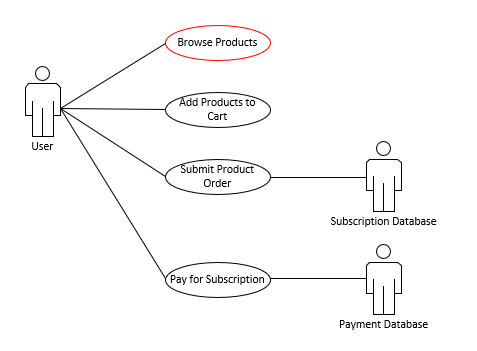
\includegraphics[scale=0.5]{UseCaseDiagrams}
	\item System Workflows using Activity Diagrams
	\newline
	Activity diagrams show how the system will accomplish the requirements set out in the user case diagrams. High-level actions are linked together to represent a process that needs to occur in the system \cite{Lamport:UML}.
	\newline
	The figure below shows an activity diagram from our class project.
	\newline
	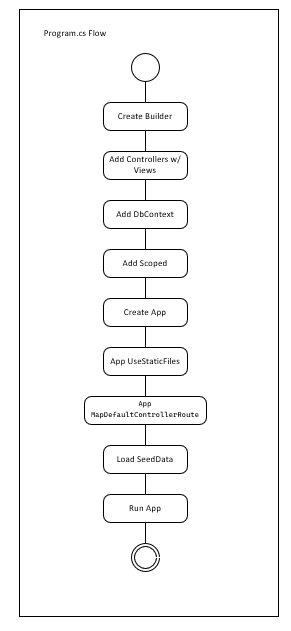
\includegraphics[scale=0.5]{ActivityDiagram}
	\item A Systems Logical Structure using Class Diagrams
	\newline
	Class diagrams show classes and their relationships \cite{Lamport:UML}.
	\newline
	The figure below shows a class diagram from our class project.
	\newline
	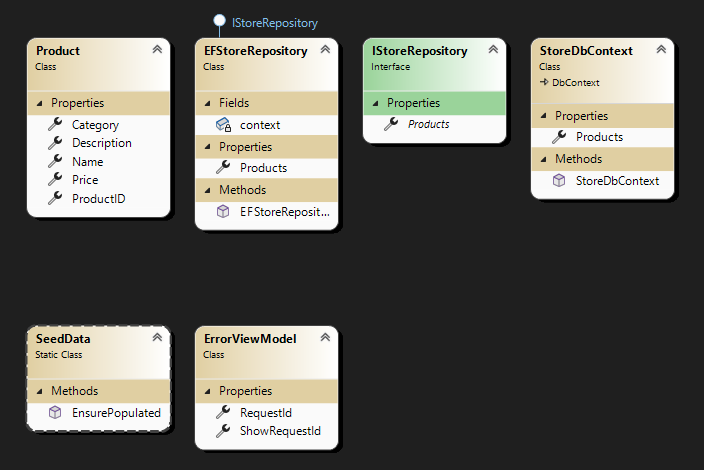
\includegraphics[scale=0.4]{ClassDiagrams}
	\item Ordered Interactions using Sequence Diagrams
	\newline
	Sequence diagrams are an important member of a group known as interaction diagrams. They help accurately model how the parts that make up the system interact.  They capture the order of interactions between parts of the system, describe which interactions will be triggered and in what order those interactions will occur.
	\newline
	The figure below shows a sequence diagram from our class project.
	\newline
	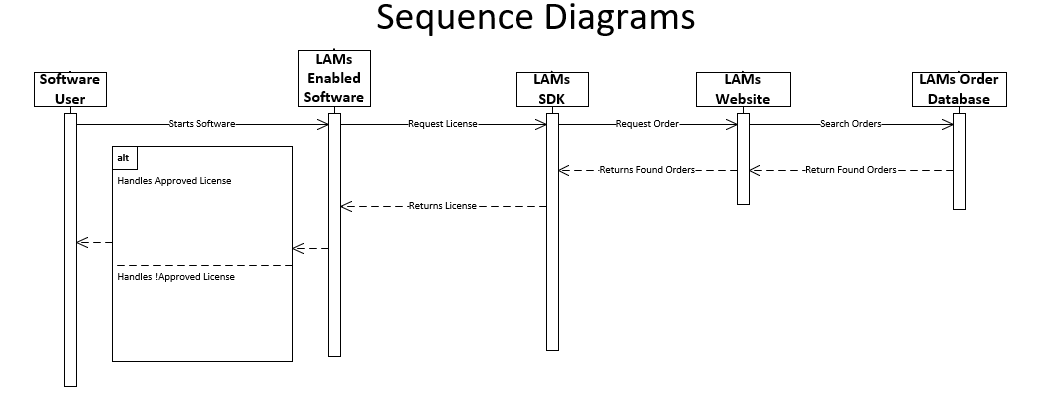
\includegraphics[scale=0.3]{SequenceDiagram}
	\item Interaction Links using Communication Diagrams
	\item Interaction Timing using Timing Diagrams
	\item Interaction Picture using Interaction Overview Diagrams
	\item Internal Class Structure using Composite Structures
	\item System Parts using Component Diagrams
	\item Organize Your Model using Packages
	\item Object State using State Machine Diagrams
	\item The Deployed System using Deployment Diagrams
\end{enumerate}
Wiegers and Beatty discuss the importance of using both textual and visual formats to capture the full intentions of the intended system. Their book describes the following visual requirements models \cite{Lamport:SoftwareRequirements}.
\begin{enumerate}
	\item Data flow diagrams (DFDs)
	\item Process flow diagrams 
	\item State-transition diagrams and state tables
	\item Dialog maps
	\item Decision tables and decision trees
	\item Event-response tables
	\item Feature trees (Ch 5)
	\item Use case diagrams (Ch 8)
	\item Activity diagrams (Ch 8)
	\item Entity-relationship diagrams (Ch 13)
\end{enumerate}
Wiegers and Beatty also briefly discuss the use of visual models in agile driven projects \cite{Lamport:SoftwareRequirements}.

Weilkiens introduces a toolbox that can be used for modeling complex and distributed systems called SYSMOD. This toolbox helps to alleviate some of the problems due to rising complexity of systems. There is a great need to express component systems in a way that can be easily shared between team members. A shared language is important for being able to complete the design task \cite{Lamport:SysML}.

The American Institute of Architects discuss the need for standard content and graphics to be used by Construction Architects to document their projects (Appendix E). \cite{Lamport:AIA_Graphical_Standards}. Although software architecture and construction architecture are technically different fields, they share many common goals of turning stakeholder ideas into a real products.
\newline
The US CAD Standard (NCS) is a compilation of related documents published by several organizations for the purposes of creating a national standard for construction related CAD documents. \cite{Lamport:AIA_Graphical_Standards}.\newline
A national CAD standard provides the following advantages \cite{Lamport:AIA_Graphical_Standards}
\begin{enumerate}
	\item Allows information to be transfered throughout the project cycle from one professional to another.
	\item Results in better coordination between architects and engineers
	\item Saves production time
	\item Improves the overall design of the project
\end{enumerate}
The Uniform Drawing System consist of 8 modules that help standardize the documents needed to convey information from the architect to the builder \cite{Lamport:AIA_Graphical_Standards}.
\begin{enumerate}
	\item Module 1 - Drawing Set Organization
	\item Module 2 - Sheet Organization
	\item Module 3 - Schedules
	\item Module 4 - Drafting Conventions
	\item Module 5 - Terms and Abbreviations
	\item Module 6 - Symbols
	\item Module 7 - Notations
	\item Module 8 - Code Conventions
\end{enumerate}

Of particular interest is the recommendation of using of a drawing set hierarchy in the NCS.  

Ingeno discusses methods for documenting and reviewing software architectures \cite{Lamport:SoftwareArchitectureHandbook} In particular, he discusses
\begin{enumerate}
	\item Uses of software architecture documentation
	\item Creating architecture descriptions (ADs), including architecture views
	\item Using UML to document software architecture
	\item Reviewing software architecture documents
\end{enumerate}

\section{Proposed Approach}
A table will be generated showing which format is recommended by each professional or professional association.

\section{Experimental Results}
Table 1 summarizes the opinions of various experts in the field of technical documentation.
\begin{table}[ht]
	\caption{Expert Recommendations for Document Formats} % title of Table
	\centering % used for centering table
	\begin{tabular}{c c c c} % centered columns (4 columns)
		\hline\hline %inserts double horizontal lines
		Expert & Text & Graphics & Both \\ [0.5ex] % inserts table
		%heading
		\hline % inserts single horizontal line
		Miles and Hamilton \cite{Lamport:UML} &  &  & Yes \\ % inserting body of the table
		Wiegers and Beatty \cite{Lamport:SoftwareRequirements} &  &  & Yes \\
		Weilkiens \cite{Lamport:SysML} &  &  & Yes \\
		Ingeno \cite{Lamport:SoftwareArchitectureHandbook} &  &  & Yes \\
		Lamsweerde \cite{Lamport:RequirementsEngineering} &  &  & Yes \\
		AIA \cite{Lamport:AIA_Graphical_Standards} &  &  & Yes \\
		NCS \cite{NCS} &  &  & Yes \\ [1ex] % [1ex] adds vertical space
		\hline %inserts single line
	\end{tabular}
	\label{table:nonlin} % is used to refer this table in the text
\end{table}

\section{Discussion}


\section{Threats to Validity}

\section{Conclusions and Future Work}
Because natural language specifications can result in incomplete and/or inaccurate application builds, natural language only specifications should be limited to the following circumstances.
\begin{enumerate}
	\item Throw away protypes used for evaluation purposes only.
	\item Applications that will not evolve over time.
	\item Applications that do not involve safety, reliability, or finances.
	\item Applications that will not require maintenance.
\end{enumerate}
Due to the fact that most applications need to both evolve over time and will eventually require maintenance, our conclusion is that the majority of software specifications need to include both natural language and graphical representations to fully document their functionality. This will lead to more complete and accurate implementation of specifications by software developers. The only real exception to this is for quick and dirty prototypes that will be discarded after their usefulness has expired.

\section{Acknowledgments}
We would like to thank Dr. Kristen Walcott, Dr. Armin Moin and the Computer Science and Software Engineering Department at UCCS for helping us gain a deeper understanding of the challenges and opportunities in software architecture.

\section{Notes and Brainstorming - Delete before submitting final paper}
\begin{enumerate}
	\item Understanding Research Problems
	\begin{enumerate}
		\item Topic: We are evaluating the usefulness of presenting ideas in different formats 
		\item Question: because we want to find out if certain formats are more useful than others in communicating ideas from stakeholders to software developers
		\item Significance: so that we can help others choose a document format that will result in successful communication of ideas from stakeholders to software developers. 
	\end{enumerate}
	\item Levels of Idea Formats from Abstract to Concrete
	\begin{enumerate}
		\item Mental
		\item Natural Language
		\begin{enumerate}
			\item Oral
			\item Written
		\end{enumerate}
			
		\item Formal Languages
		\begin{enumerate}
			\item Mathematical
			\item Models (UML)
		\end{enumerate}
		\item Source Code
	\end{enumerate}
\end{enumerate}

 
%
% The following two commands are all you need in the
% initial runs of your .tex file to
% produce the bibliography for the citations in your paper.
\bibliographystyle{abbrv}
\bibliography{sigproc}  % sigproc.bib is the name of the Bibliography in this case
% You must have a proper ".bib" file
%  and remember to run:
% latex bibtex latex latex
% to resolve all references
%
% ACM needs 'a single self-contained file'!
%

\balancecolumns
% That's all folks!
\end{document}
